\begin{figure*}[t]
\centering
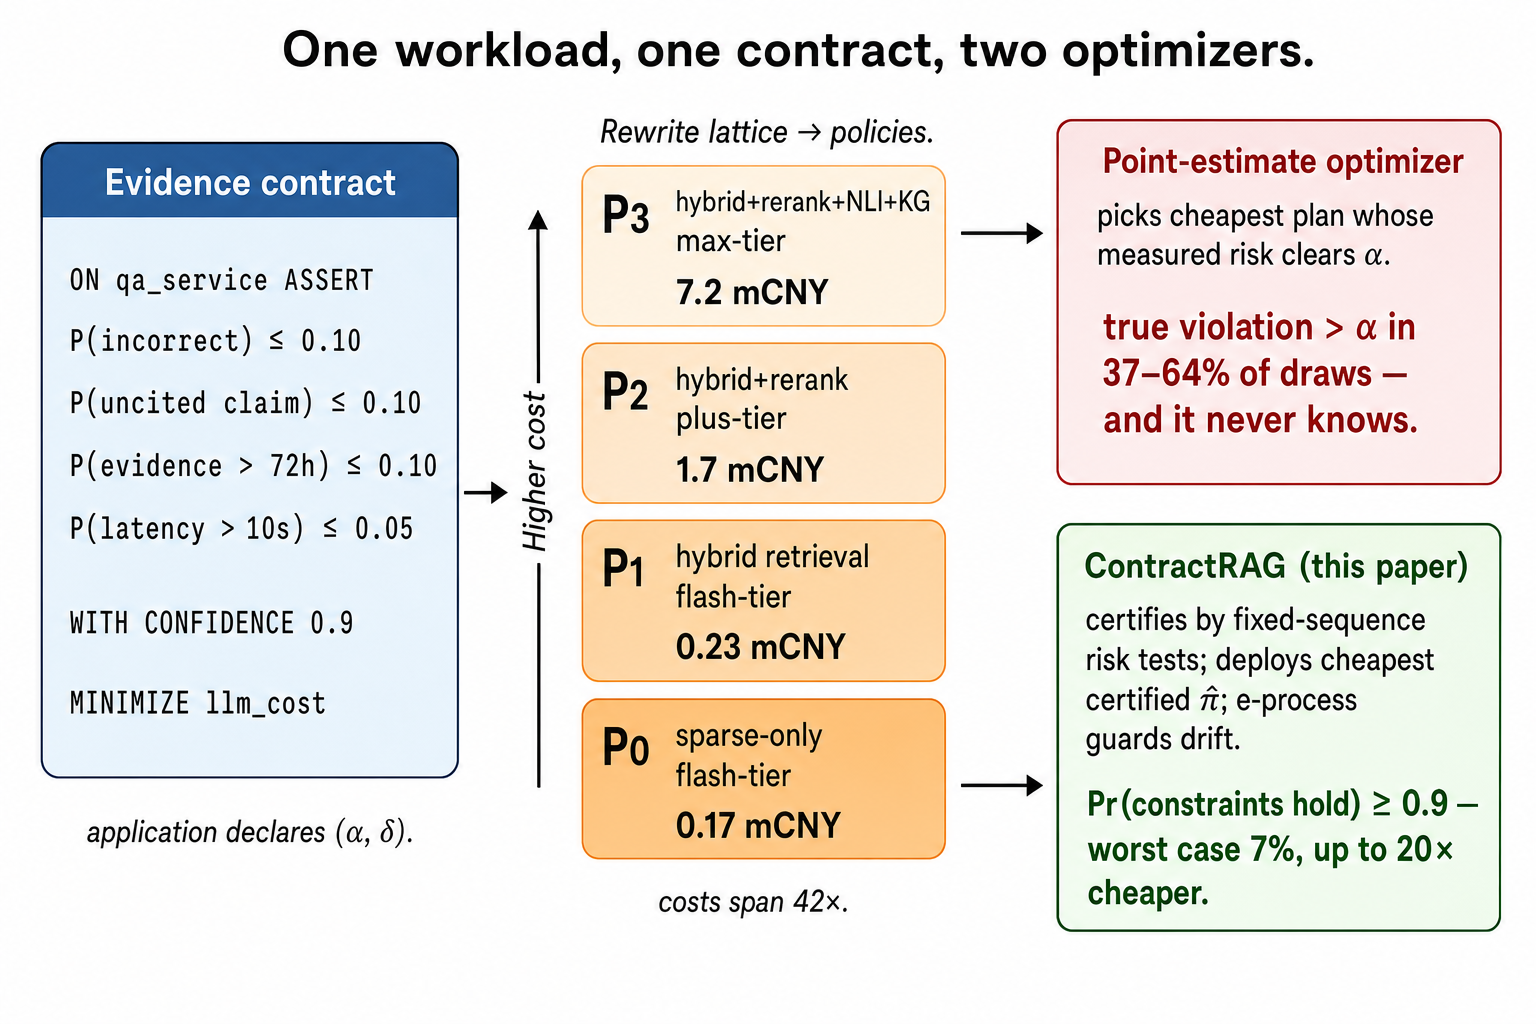
\includegraphics[width=\textwidth]{figures/fig_example_imagegen.png}
\caption{One workload, one contract, two optimizers. (Left) the
application declares admissible violation rates for correctness,
citations, freshness, and latency, plus a certification budget
$\delta=0.1$. (Center) cost-decreasing rewrites induce a space of plans
and per-query adaptive policies whose costs span 42$\times$. (Right) a
state-of-practice optimizer compares point estimates against the
constraint and routinely deploys infeasible plans; \system\ deploys the
cheapest policy that \emph{passes a statistical feasibility test}, so
the contract holds with probability $\ge 1-\delta$ for any query
distribution (Theorem~\ref{thm:validity}).}
\label{fig:example}
\end{figure*}
